\documentclass[]{article}
\usepackage{lmodern}
\usepackage{amssymb,amsmath}
\usepackage{ifxetex,ifluatex}
\usepackage{fixltx2e} % provides \textsubscript
\ifnum 0\ifxetex 1\fi\ifluatex 1\fi=0 % if pdftex
  \usepackage[T1]{fontenc}
  \usepackage[utf8]{inputenc}
\else % if luatex or xelatex
  \ifxetex
    \usepackage{mathspec}
  \else
    \usepackage{fontspec}
  \fi
  \defaultfontfeatures{Ligatures=TeX,Scale=MatchLowercase}
\fi
% use upquote if available, for straight quotes in verbatim environments
\IfFileExists{upquote.sty}{\usepackage{upquote}}{}
% use microtype if available
\IfFileExists{microtype.sty}{%
\usepackage{microtype}
\UseMicrotypeSet[protrusion]{basicmath} % disable protrusion for tt fonts
}{}
\usepackage[margin=1in]{geometry}
\usepackage{hyperref}
\hypersetup{unicode=true,
            pdftitle={STA 521 - Final Project Part I},
            pdfauthor={FP-Team 01: Qianyin Lu, George Lindner, Chenxi Wu, Yi Mi},
            pdfborder={0 0 0},
            breaklinks=true}
\urlstyle{same}  % don't use monospace font for urls
\usepackage{color}
\usepackage{fancyvrb}
\newcommand{\VerbBar}{|}
\newcommand{\VERB}{\Verb[commandchars=\\\{\}]}
\DefineVerbatimEnvironment{Highlighting}{Verbatim}{commandchars=\\\{\}}
% Add ',fontsize=\small' for more characters per line
\usepackage{framed}
\definecolor{shadecolor}{RGB}{248,248,248}
\newenvironment{Shaded}{\begin{snugshade}}{\end{snugshade}}
\newcommand{\AlertTok}[1]{\textcolor[rgb]{0.94,0.16,0.16}{#1}}
\newcommand{\AnnotationTok}[1]{\textcolor[rgb]{0.56,0.35,0.01}{\textbf{\textit{#1}}}}
\newcommand{\AttributeTok}[1]{\textcolor[rgb]{0.77,0.63,0.00}{#1}}
\newcommand{\BaseNTok}[1]{\textcolor[rgb]{0.00,0.00,0.81}{#1}}
\newcommand{\BuiltInTok}[1]{#1}
\newcommand{\CharTok}[1]{\textcolor[rgb]{0.31,0.60,0.02}{#1}}
\newcommand{\CommentTok}[1]{\textcolor[rgb]{0.56,0.35,0.01}{\textit{#1}}}
\newcommand{\CommentVarTok}[1]{\textcolor[rgb]{0.56,0.35,0.01}{\textbf{\textit{#1}}}}
\newcommand{\ConstantTok}[1]{\textcolor[rgb]{0.00,0.00,0.00}{#1}}
\newcommand{\ControlFlowTok}[1]{\textcolor[rgb]{0.13,0.29,0.53}{\textbf{#1}}}
\newcommand{\DataTypeTok}[1]{\textcolor[rgb]{0.13,0.29,0.53}{#1}}
\newcommand{\DecValTok}[1]{\textcolor[rgb]{0.00,0.00,0.81}{#1}}
\newcommand{\DocumentationTok}[1]{\textcolor[rgb]{0.56,0.35,0.01}{\textbf{\textit{#1}}}}
\newcommand{\ErrorTok}[1]{\textcolor[rgb]{0.64,0.00,0.00}{\textbf{#1}}}
\newcommand{\ExtensionTok}[1]{#1}
\newcommand{\FloatTok}[1]{\textcolor[rgb]{0.00,0.00,0.81}{#1}}
\newcommand{\FunctionTok}[1]{\textcolor[rgb]{0.00,0.00,0.00}{#1}}
\newcommand{\ImportTok}[1]{#1}
\newcommand{\InformationTok}[1]{\textcolor[rgb]{0.56,0.35,0.01}{\textbf{\textit{#1}}}}
\newcommand{\KeywordTok}[1]{\textcolor[rgb]{0.13,0.29,0.53}{\textbf{#1}}}
\newcommand{\NormalTok}[1]{#1}
\newcommand{\OperatorTok}[1]{\textcolor[rgb]{0.81,0.36,0.00}{\textbf{#1}}}
\newcommand{\OtherTok}[1]{\textcolor[rgb]{0.56,0.35,0.01}{#1}}
\newcommand{\PreprocessorTok}[1]{\textcolor[rgb]{0.56,0.35,0.01}{\textit{#1}}}
\newcommand{\RegionMarkerTok}[1]{#1}
\newcommand{\SpecialCharTok}[1]{\textcolor[rgb]{0.00,0.00,0.00}{#1}}
\newcommand{\SpecialStringTok}[1]{\textcolor[rgb]{0.31,0.60,0.02}{#1}}
\newcommand{\StringTok}[1]{\textcolor[rgb]{0.31,0.60,0.02}{#1}}
\newcommand{\VariableTok}[1]{\textcolor[rgb]{0.00,0.00,0.00}{#1}}
\newcommand{\VerbatimStringTok}[1]{\textcolor[rgb]{0.31,0.60,0.02}{#1}}
\newcommand{\WarningTok}[1]{\textcolor[rgb]{0.56,0.35,0.01}{\textbf{\textit{#1}}}}
\usepackage{graphicx,grffile}
\makeatletter
\def\maxwidth{\ifdim\Gin@nat@width>\linewidth\linewidth\else\Gin@nat@width\fi}
\def\maxheight{\ifdim\Gin@nat@height>\textheight\textheight\else\Gin@nat@height\fi}
\makeatother
% Scale images if necessary, so that they will not overflow the page
% margins by default, and it is still possible to overwrite the defaults
% using explicit options in \includegraphics[width, height, ...]{}
\setkeys{Gin}{width=\maxwidth,height=\maxheight,keepaspectratio}
\IfFileExists{parskip.sty}{%
\usepackage{parskip}
}{% else
\setlength{\parindent}{0pt}
\setlength{\parskip}{6pt plus 2pt minus 1pt}
}
\setlength{\emergencystretch}{3em}  % prevent overfull lines
\providecommand{\tightlist}{%
  \setlength{\itemsep}{0pt}\setlength{\parskip}{0pt}}
\setcounter{secnumdepth}{0}
% Redefines (sub)paragraphs to behave more like sections
\ifx\paragraph\undefined\else
\let\oldparagraph\paragraph
\renewcommand{\paragraph}[1]{\oldparagraph{#1}\mbox{}}
\fi
\ifx\subparagraph\undefined\else
\let\oldsubparagraph\subparagraph
\renewcommand{\subparagraph}[1]{\oldsubparagraph{#1}\mbox{}}
\fi

%%% Use protect on footnotes to avoid problems with footnotes in titles
\let\rmarkdownfootnote\footnote%
\def\footnote{\protect\rmarkdownfootnote}

%%% Change title format to be more compact
\usepackage{titling}

% Create subtitle command for use in maketitle
\providecommand{\subtitle}[1]{
  \posttitle{
    \begin{center}\large#1\end{center}
    }
}

\setlength{\droptitle}{-2em}

  \title{STA 521 - Final Project Part I}
    \pretitle{\vspace{\droptitle}\centering\huge}
  \posttitle{\par}
    \author{FP-Team 01: Qianyin Lu, George Lindner, Chenxi Wu, Yi Mi}
    \preauthor{\centering\large\emph}
  \postauthor{\par}
      \predate{\centering\large\emph}
  \postdate{\par}
    \date{December 7th, 2019}

\usepackage{booktabs}
\usepackage{longtable}
\usepackage{array}
\usepackage{multirow}
\usepackage{wrapfig}
\usepackage{float}
\usepackage{colortbl}
\usepackage{pdflscape}
\usepackage{tabu}
\usepackage{threeparttable}
\usepackage{threeparttablex}
\usepackage[normalem]{ulem}
\usepackage{makecell}
\usepackage{xcolor}

\begin{document}
\maketitle

\hypertarget{introduction-summary-of-problem-and-objectives}{%
\subsection{1. Introduction: Summary of problem and
objectives}\label{introduction-summary-of-problem-and-objectives}}

Our team of esteemed statisticians was recently hired by a prestigious
art historian for a consulting project. We were asked to help build a
predictive model in exchange for an A on our STA 521 Final Exam. After
much discussion, our team accepted the historian's offer.

We were given the task of predicting paintings' selling prices at
auctions in 18th century Paris. To accomplish this, we used a dataset
containing information about each painting's buyer, seller, painter, and
characteristics of the painting. These variables were all possible
predictor variables in modeling the response variable, the selling price
of a painting.

There were two primary objectives in our analysis:

\begin{enumerate}
\def\labelenumi{\arabic{enumi})}
\tightlist
\item
  To determine which variables (or interactions) drove the price of a
  painting
\item
  To determine which paintings were overpriced or and which were
  underpriced.
\end{enumerate}

After arriving at a final model, we are able to answer these primary
questions. Any variables that appear in the model will be important in
driving painting prices, and observing residuals will enable us to
determine if a painting was over or underpriced.

We had 1,500 observations to train the model on, along with 750
observations held out as a testing set. There were a total of 59
variables in the dataset, both categorical and continuous.

\hypertarget{exploratory-data-analysis}{%
\subsection{2. Exploratory Data
Analysis:}\label{exploratory-data-analysis}}

\hypertarget{initial-data-cleaning}{%
\subsubsection{Initial Data Cleaning}\label{initial-data-cleaning}}

We began our data cleaning process by reading the codebook for a better
understanding of what each variable in the data represented. Several
predictors in the dataset were redundant and therefore removed to avoid
high correlation among the predictors. Examples of this include the
variable \emph{sale}, which is a combination of \emph{dealer} and
\emph{year}. Additionally, there were other predictors that we deemed
would not be useful for prediction, such as \emph{count} which was 1 for
every observation, or \emph{subject} which was a short description of
the content in the painting. We simplified the data by eliminating
unnecessary predictors.

\hypertarget{categorical-variables}{%
\subsubsection{Categorical Variables}\label{categorical-variables}}

We recoded each categorical variable to be a factor. We created a
visualization of the binary categorical variables to observe the balance
between classes below.

\hypertarget{plot-1}{%
\subsubsection{Plot 1}\label{plot-1}}

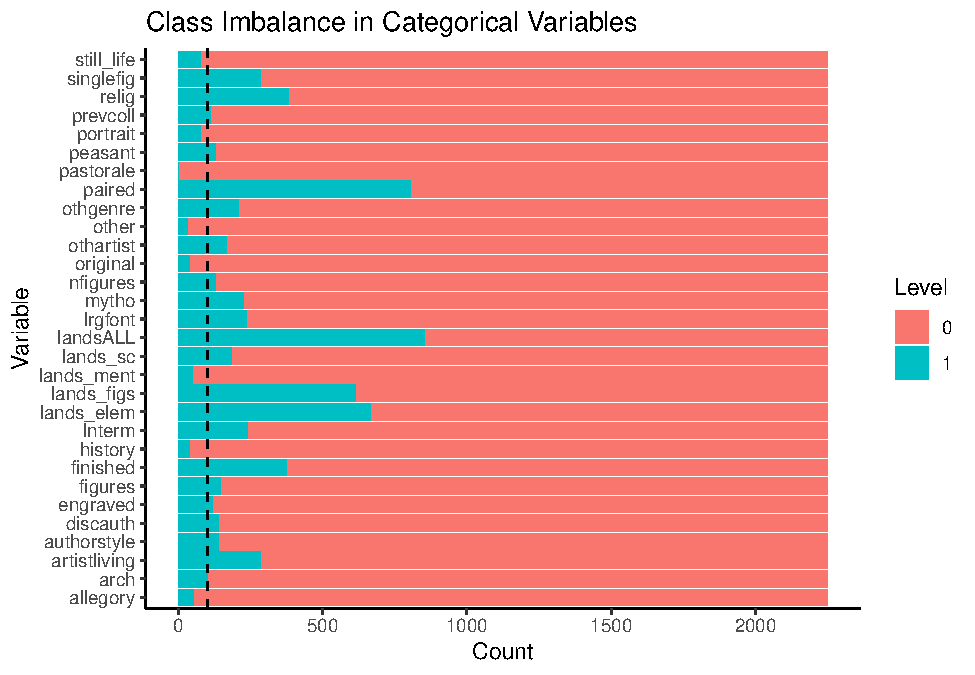
\includegraphics{Part-I-Writeup_files/figure-latex/unnamed-chunk-1-1.pdf}
Imbalanced classes can lead to poor \(\beta\) estimates if the
underrepresented class does not have enough data. This was our
motivation to remove any variable that had less than an arbitrary 100
observations in a class, which is denoted by the dotted black line in
our visualization above.

To identify important categorical variables, we created a boxplot for
each variable that compared the distribution of \emph{logprice} over
every level of the factor. The results are shown below.

\hypertarget{plot-2}{%
\subsubsection{Plot 2}\label{plot-2}}

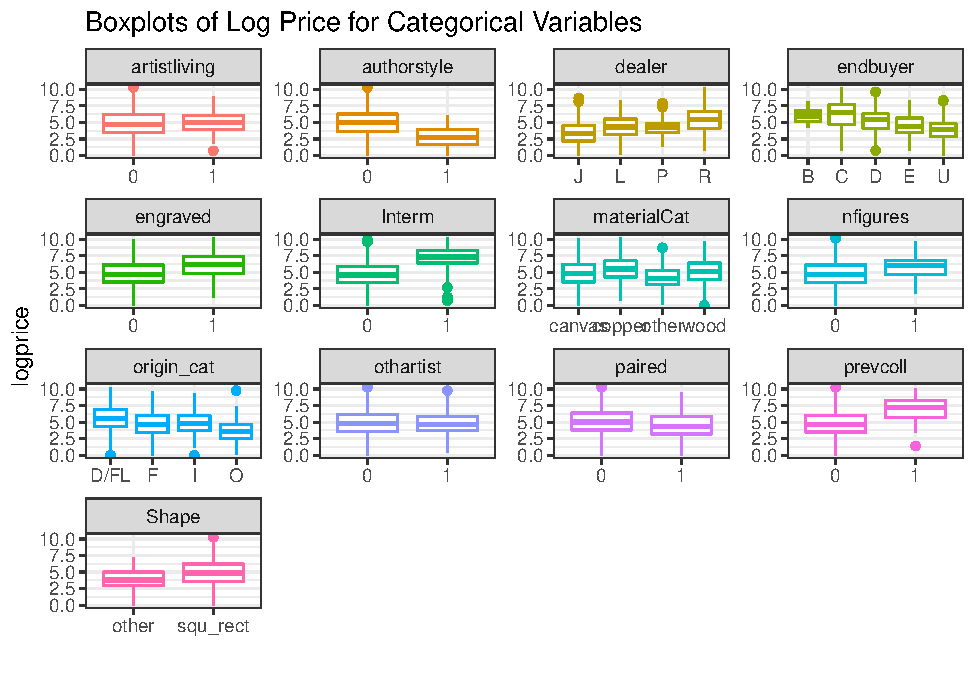
\includegraphics{Part-I-Writeup_files/figure-latex/eda-1.pdf}
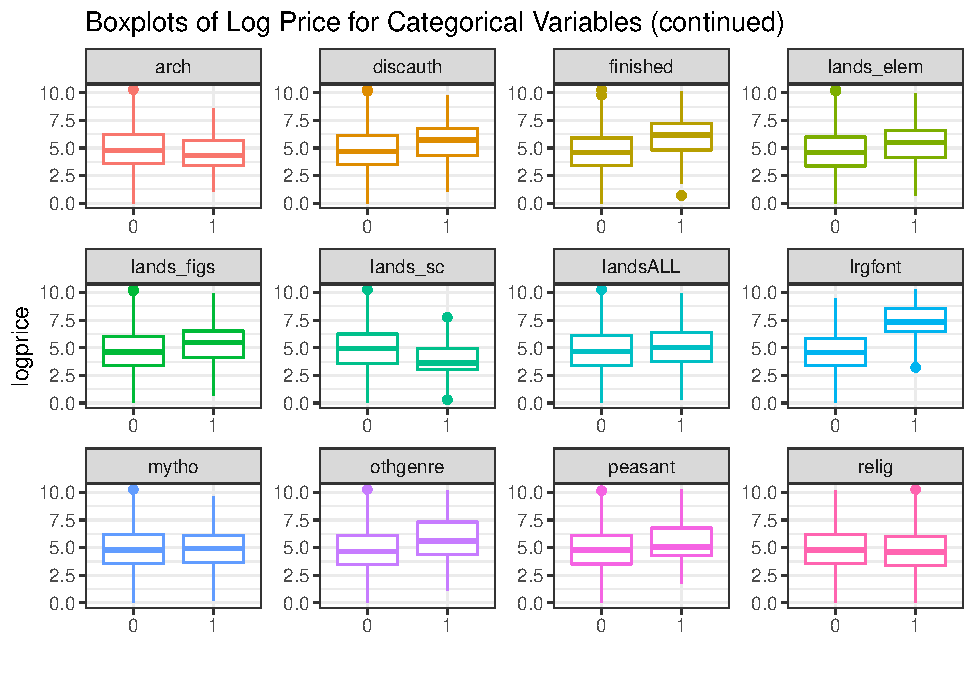
\includegraphics{Part-I-Writeup_files/figure-latex/eda-2.pdf}

The boxplots above help us identify which variables could be important
in predicting a painting's price. They also help us in our variable
selection process by displaying variables that have similar prices in
all of their categories. After inspecting the boxplots, we determined
that \emph{mytho}, \emph{landsALL}, \emph{relig}, and \emph{othartist}
were not useful for prediction. Variables that may be important include,
but are not limited to, \emph{lrgfont}, \emph{Interm},
\emph{authorstyle}, and \emph{prevcoll}.

\hypertarget{quantitative-variables}{%
\subsubsection{Quantitative Variables}\label{quantitative-variables}}

There are also quantitative variables in our data that could be used for
prediction. Like the categorical variables, many of these predictors
were redundant. For example, we were given the surface area of a
painting. Additionally, we were given a variable for surface area if the
painting was round and a surface area variable if the painting was
rectangular. We also were given the height, the width, and the diameter
of the painting. We determined that all this information could be
condensed to a single variable, \emph{Surface}.

There was missing data in \emph{Surface} that we had to address. Surface
area intuitively seems like it could drive the price of a painting, so
we had to develop a strategy for handling the missing observations. With
the help of the plot below, we determined that imputing the median
surface area size of the dataset would be a good estimation for missing
values. Since the distribution of \emph{Surface} is skewed, we wanted an
imputation strategy that would be robust to outliers. Thus, we opted for
the median over the mean.

\hypertarget{plot-3}{%
\subsubsection{Plot 3}\label{plot-3}}

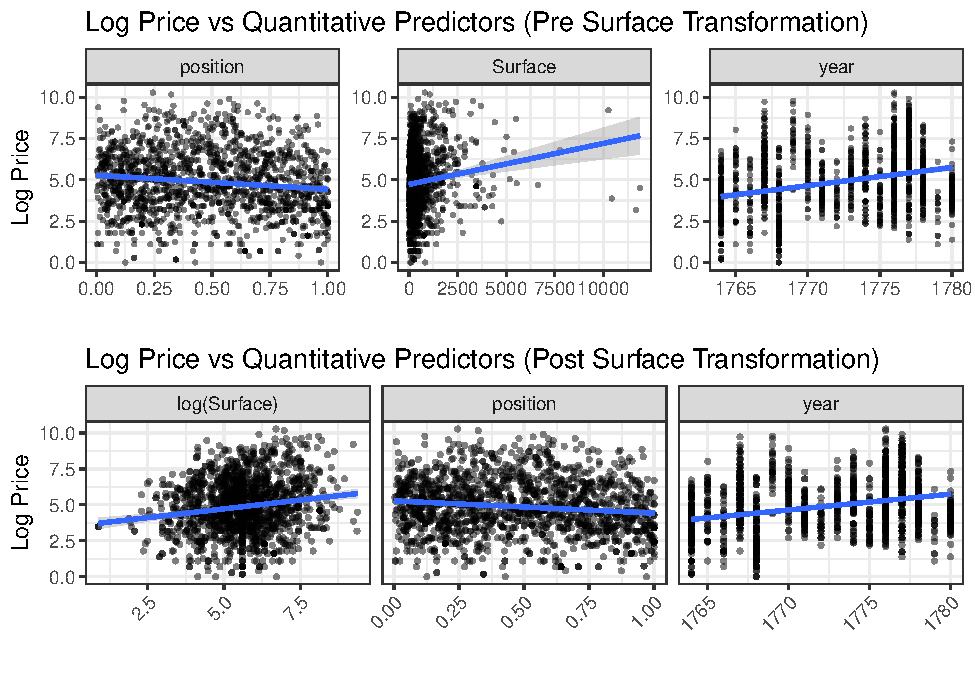
\includegraphics{Part-I-Writeup_files/figure-latex/unnamed-chunk-2-1.pdf}

We created scatterplots to observe the relationship between our three
quantitative predictor variables and the log price of a painting. The
distribution of \emph{Surface} was skewed right and a log transformation
was necessary. We plot the relationship of logprice and the transformed
Surface column in the lower graph.

After considering our EDA plots, we determined the 10 variables that we
thought would be most useful in predicting \emph{logprice}.

\begin{table}

\caption{\label{tab:kable important variables}10 Most Important Predictor Variables, from EDA}
\centering
\begin{tabular}[t]{r|l}
\hline
Rank & Variable\\
\hline
1 & log(Surface)\\
\hline
2 & lrgfont\\
\hline
3 & Interm\\
\hline
4 & authorstyle\\
\hline
5 & prevcoll\\
\hline
6 & origin\_cat\\
\hline
7 & engraved\\
\hline
8 & finished\\
\hline
9 & discauth\\
\hline
10 & dealer\\
\hline
\end{tabular}
\end{table}

With the data cleaned and important variables identified, we move to the
next step of the process: modeling the data.

\hypertarget{development-and-assessment-of-initial-model}{%
\subsubsection{3. Development and Assessment of Initial
Model:}\label{development-and-assessment-of-initial-model}}

\begin{Shaded}
\begin{Highlighting}[]
\CommentTok{# use bic to select the variables which could be used to build interaction terms}
\NormalTok{model}\FloatTok{.0}\NormalTok{ <-}\StringTok{ }\KeywordTok{lm}\NormalTok{(logprice }\OperatorTok{~}\StringTok{ }\NormalTok{position }\OperatorTok{+}\StringTok{ }\NormalTok{dealer }\OperatorTok{+}\StringTok{ }\NormalTok{year }\OperatorTok{+}\StringTok{ }\NormalTok{origin_cat }\OperatorTok{+}\StringTok{ }\NormalTok{artistliving }\OperatorTok{+}\StringTok{ }
\StringTok{    }\NormalTok{authorstyle }\OperatorTok{+}\StringTok{ }\NormalTok{endbuyer }\OperatorTok{+}\StringTok{ }\NormalTok{Interm }\OperatorTok{+}\StringTok{ }\NormalTok{Shape }\OperatorTok{+}\StringTok{ }\KeywordTok{log}\NormalTok{(Surface) }\OperatorTok{+}\StringTok{ }\NormalTok{materialCat }\OperatorTok{+}\StringTok{ }
\StringTok{    }\NormalTok{nfigures }\OperatorTok{+}\StringTok{ }\NormalTok{engraved }\OperatorTok{+}\StringTok{ }\NormalTok{prevcoll }\OperatorTok{+}\StringTok{ }\NormalTok{paired }\OperatorTok{+}\StringTok{ }\NormalTok{finished }\OperatorTok{+}\StringTok{ }\NormalTok{lrgfont }\OperatorTok{+}\StringTok{ }
\StringTok{    }\NormalTok{lands_sc }\OperatorTok{+}\StringTok{ }\NormalTok{lands_elem }\OperatorTok{+}\StringTok{ }\NormalTok{lands_figs }\OperatorTok{+}\StringTok{ }\NormalTok{arch }\OperatorTok{+}\StringTok{ }\NormalTok{peasant }\OperatorTok{+}\StringTok{ }\NormalTok{othgenre }\OperatorTok{+}\StringTok{ }
\StringTok{    }\NormalTok{discauth, }\DataTypeTok{data =}\NormalTok{ paint_train)}

\CommentTok{# summary(model.0)}

\NormalTok{model.}\FloatTok{0.}\NormalTok{bic =}\StringTok{ }\KeywordTok{step}\NormalTok{(model}\FloatTok{.0}\NormalTok{, }\DataTypeTok{k=}\KeywordTok{log}\NormalTok{(}\KeywordTok{nrow}\NormalTok{(paint_train)), }\DataTypeTok{trace =}\NormalTok{ F)}

\CommentTok{# summary(model.0.bic)}

\CommentTok{# use the resulting fomula of bic to find interactions with aic}

\NormalTok{model}\FloatTok{.1}\NormalTok{ =}\StringTok{ }\KeywordTok{lm}\NormalTok{(}\DataTypeTok{formula =}\NormalTok{ logprice }\OperatorTok{~}\StringTok{ }\NormalTok{(dealer }\OperatorTok{+}\StringTok{ }\NormalTok{year }\OperatorTok{+}\StringTok{ }\NormalTok{origin_cat }\OperatorTok{+}\StringTok{ }\NormalTok{artistliving }\OperatorTok{+}\StringTok{ }
\StringTok{    }\NormalTok{authorstyle }\OperatorTok{+}\StringTok{ }\NormalTok{endbuyer }\OperatorTok{+}\StringTok{ }\NormalTok{Interm }\OperatorTok{+}\StringTok{ }\KeywordTok{log}\NormalTok{(Surface) }\OperatorTok{+}\StringTok{ }\NormalTok{engraved }\OperatorTok{+}\StringTok{ }\NormalTok{prevcoll }\OperatorTok{+}\StringTok{ }
\StringTok{    }\NormalTok{paired }\OperatorTok{+}\StringTok{ }\NormalTok{finished }\OperatorTok{+}\StringTok{ }\NormalTok{lrgfont }\OperatorTok{+}\StringTok{ }\NormalTok{lands_sc }\OperatorTok{+}\StringTok{ }\NormalTok{discauth)}\OperatorTok{^}\DecValTok{2}\NormalTok{, }\DataTypeTok{data =}\NormalTok{ paint_train)}

\NormalTok{model.}\FloatTok{1.}\NormalTok{aic =}\StringTok{ }\KeywordTok{step}\NormalTok{(model}\FloatTok{.1}\NormalTok{, }\DataTypeTok{k =} \DecValTok{2}\NormalTok{, }\DataTypeTok{trace =}\NormalTok{ F)}

\CommentTok{#summary(model.1.aic)}

\CommentTok{#plot(model.1.aic)}
\end{Highlighting}
\end{Shaded}

We first remove some variables because they have very similar levels and
thus may not have significant influence on the response.

We use BIC to select the important variables. And we use the BIC result
to build a new model and construct all interaction terms and then we use
AIC to determine the final model.(may not appear in the write-up for bic
part)

We deleted some interactions for the follow reasons. We deleted the
interactions \texttt{lands\_sc:discauth}, \texttt{paired:lands\_sc} and
\texttt{artistliving:lands\_sc}. First of all, for the interactions
related to \texttt{lands\_sc}, we think the \texttt{lands\_sc}--if
described as a plain landscape, is a variable describing a single
dimension of painting content and we don't think it will interact with
the variables describing the dealers' behaviour, the pairing of a
painting, or the living info of the artists. Though the Adjusted
R-squared decreased a little, from 0.66 to 0.659, we think it worth to
make the model more reasonable.

\begin{Shaded}
\begin{Highlighting}[]
\NormalTok{model1 <-}\StringTok{ }\KeywordTok{lm}\NormalTok{(}\DataTypeTok{formula =}\NormalTok{ logprice }\OperatorTok{~}\StringTok{ }\NormalTok{dealer }\OperatorTok{+}\StringTok{ }\NormalTok{year }\OperatorTok{+}\StringTok{ }\NormalTok{origin_cat }\OperatorTok{+}\StringTok{ }\NormalTok{artistliving }\OperatorTok{+}\StringTok{ }
\StringTok{                   }\NormalTok{authorstyle }\OperatorTok{+}\StringTok{ }\NormalTok{endbuyer }\OperatorTok{+}\StringTok{ }\NormalTok{Interm }\OperatorTok{+}\StringTok{ }\KeywordTok{log}\NormalTok{(Surface) }\OperatorTok{+}\StringTok{ }\NormalTok{engraved }\OperatorTok{+}\StringTok{ }\NormalTok{prevcoll }\OperatorTok{+}
\StringTok{                   }\NormalTok{paired }\OperatorTok{+}\StringTok{ }\NormalTok{finished }\OperatorTok{+}\StringTok{ }\NormalTok{lrgfont }\OperatorTok{+}\StringTok{ }\NormalTok{lands_sc }\OperatorTok{+}\StringTok{ }\NormalTok{discauth }\OperatorTok{+}\StringTok{ }\NormalTok{dealer}\OperatorTok{:}\NormalTok{year }\OperatorTok{+}\StringTok{ }
\StringTok{                   }\OperatorTok{+}\StringTok{ }\NormalTok{dealer}\OperatorTok{:}\NormalTok{Interm }\OperatorTok{+}\StringTok{ }\NormalTok{dealer}\OperatorTok{:}\NormalTok{discauth }\OperatorTok{+}\StringTok{ }\NormalTok{year}\OperatorTok{:}\NormalTok{artistliving }\OperatorTok{+}\StringTok{ }
\StringTok{                   }\NormalTok{year}\OperatorTok{:}\NormalTok{endbuyer }\OperatorTok{+}\StringTok{ }\NormalTok{year}\OperatorTok{:}\KeywordTok{log}\NormalTok{(Surface) }\OperatorTok{+}\StringTok{ }\NormalTok{year}\OperatorTok{:}\NormalTok{discauth }\OperatorTok{+}\StringTok{ }
\StringTok{                   }\NormalTok{artistliving}\OperatorTok{:}\NormalTok{authorstyle }\OperatorTok{+}\StringTok{ }\NormalTok{artistliving}\OperatorTok{:}\NormalTok{discauth }\OperatorTok{+}\StringTok{ }
\StringTok{                   }\NormalTok{authorstyle}\OperatorTok{:}\KeywordTok{log}\NormalTok{(Surface) }\OperatorTok{+}\StringTok{ }\NormalTok{endbuyer}\OperatorTok{:}\NormalTok{finished }\OperatorTok{+}\StringTok{ }
\StringTok{                   }\NormalTok{endbuyer}\OperatorTok{:}\NormalTok{discauth }\OperatorTok{+}\StringTok{ }\NormalTok{Interm}\OperatorTok{:}\KeywordTok{log}\NormalTok{(Surface) }\OperatorTok{+}\StringTok{ }\NormalTok{Interm}\OperatorTok{:}\NormalTok{prevcoll }\OperatorTok{+}\StringTok{ }
\StringTok{                   }\NormalTok{Interm}\OperatorTok{:}\NormalTok{lrgfont }\OperatorTok{+}\StringTok{ }\NormalTok{Interm}\OperatorTok{:}\NormalTok{discauth }\OperatorTok{+}\StringTok{ }\KeywordTok{log}\NormalTok{(Surface)}\OperatorTok{:}\NormalTok{discauth }\OperatorTok{+}\StringTok{ }
\StringTok{                   }\NormalTok{prevcoll}\OperatorTok{:}\NormalTok{finished }\OperatorTok{+}\StringTok{ }\NormalTok{paired}\OperatorTok{:}\NormalTok{finished }\OperatorTok{+}\StringTok{ }
\StringTok{                   }\NormalTok{paired}\OperatorTok{:}\NormalTok{lrgfont }\OperatorTok{+}\StringTok{ }\NormalTok{paired}\OperatorTok{:}\NormalTok{discauth, }\DataTypeTok{data =}\NormalTok{ paint_train)}


\CommentTok{#plot(model1)}

\CommentTok{#summary(model1)}
\end{Highlighting}
\end{Shaded}

\hypertarget{model-assessment}{%
\subsubsection{Model Assessment}\label{model-assessment}}

\begin{Shaded}
\begin{Highlighting}[]
\CommentTok{# plot}
\KeywordTok{par}\NormalTok{(}\DataTypeTok{mfrow =} \KeywordTok{c}\NormalTok{(}\DecValTok{2}\NormalTok{, }\DecValTok{2}\NormalTok{))}
\KeywordTok{plot}\NormalTok{(model1, }\DataTypeTok{ask =} \OtherTok{FALSE}\NormalTok{)}
\end{Highlighting}
\end{Shaded}

\begin{verbatim}
## Warning: not plotting observations with leverage one:
##   218, 1129

## Warning: not plotting observations with leverage one:
##   218, 1129
\end{verbatim}

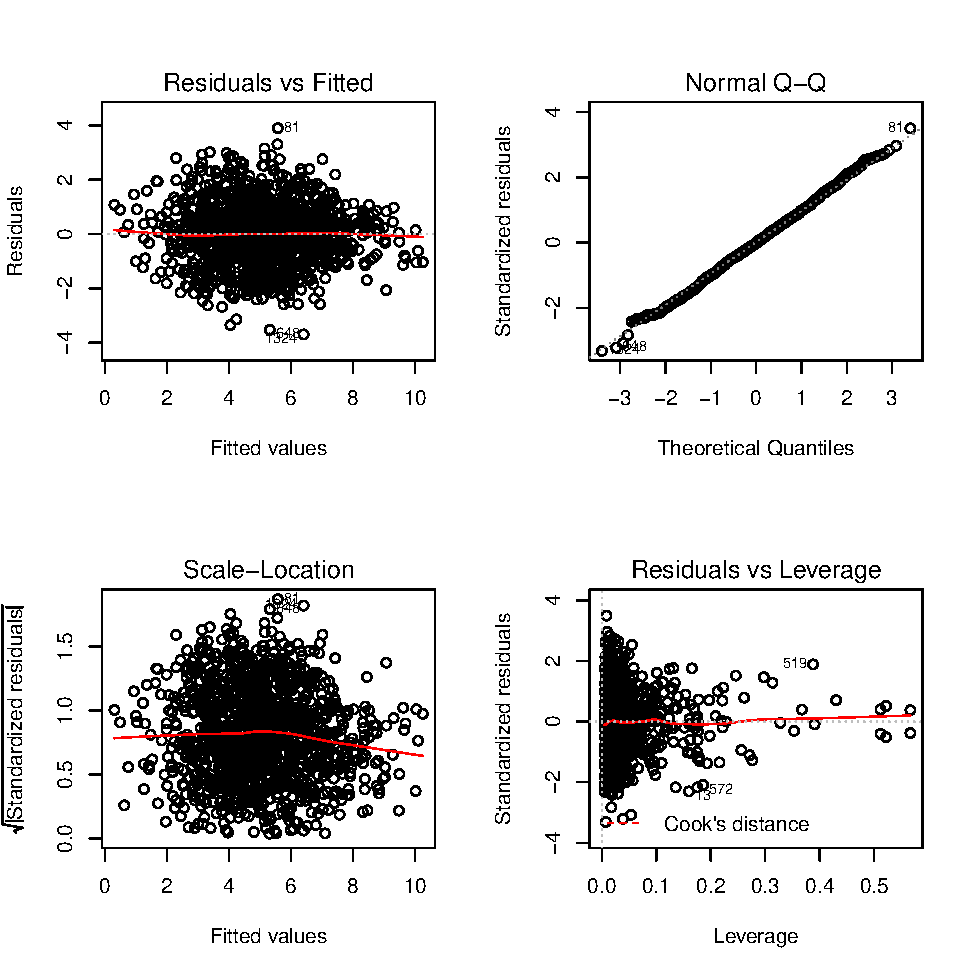
\includegraphics{Part-I-Writeup_files/figure-latex/res plot-1.pdf}

looking at the diagnostic plots, our model 1 seems to satisfy the
assumptions of linear regression resonablly well. From the Residual vs
Fitted plot we can see equally spread residuals around a horizontal line
without any distinct patterns; The Normal Q-Q plot shows the residuals
are almost normally-distributed. The Scale-Location plot shows that
homoscedasticity is met. The Residual vs Leverage plot shows that most
of the points are not influential. There are only very few points that
falls outside of Cook's distance line. The plot identified the
influential observation as \#218 and \#1129. We removed these two points
and refitted the model. But removing the two points does not improve the
R\^{}2 nor does it help with the residual diagnostics plots (See
Appendix the residual plot after refitting) So we will set Model 1 to
our final model in part-I.

\begin{Shaded}
\begin{Highlighting}[]
\CommentTok{# delete outliers and refit}
\NormalTok{paint_train_trans =}\StringTok{ }\NormalTok{paint_train[}\OperatorTok{-}\KeywordTok{c}\NormalTok{(}\DecValTok{218}\NormalTok{,}\DecValTok{1129}\NormalTok{),]}
\NormalTok{model1}\FloatTok{.1}\NormalTok{ <-}\StringTok{ }\KeywordTok{lm}\NormalTok{(}\DataTypeTok{formula =}\NormalTok{ logprice }\OperatorTok{~}\StringTok{ }\NormalTok{dealer }\OperatorTok{+}\StringTok{ }\NormalTok{year }\OperatorTok{+}\StringTok{ }\NormalTok{origin_cat }\OperatorTok{+}\StringTok{ }\NormalTok{artistliving }\OperatorTok{+}\StringTok{ }

\StringTok{                   }\NormalTok{authorstyle }\OperatorTok{+}\StringTok{ }\NormalTok{endbuyer }\OperatorTok{+}\StringTok{ }\NormalTok{Interm }\OperatorTok{+}\StringTok{ }\KeywordTok{log}\NormalTok{(Surface) }\OperatorTok{+}\StringTok{ }\NormalTok{engraved }\OperatorTok{+}\StringTok{ }\NormalTok{prevcoll }\OperatorTok{+}
\StringTok{                   }\NormalTok{paired }\OperatorTok{+}\StringTok{ }\NormalTok{finished }\OperatorTok{+}\StringTok{ }\NormalTok{lrgfont }\OperatorTok{+}\StringTok{ }\NormalTok{lands_sc }\OperatorTok{+}\StringTok{ }\NormalTok{discauth }\OperatorTok{+}\StringTok{ }\NormalTok{dealer}\OperatorTok{:}\NormalTok{year }\OperatorTok{+}\StringTok{ }
\StringTok{                   }\OperatorTok{+}\StringTok{ }\NormalTok{dealer}\OperatorTok{:}\NormalTok{Interm }\OperatorTok{+}\StringTok{ }\NormalTok{dealer}\OperatorTok{:}\NormalTok{discauth }\OperatorTok{+}\StringTok{ }\NormalTok{year}\OperatorTok{:}\NormalTok{artistliving }\OperatorTok{+}\StringTok{ }
\StringTok{                   }\NormalTok{year}\OperatorTok{:}\NormalTok{endbuyer }\OperatorTok{+}\StringTok{ }\NormalTok{year}\OperatorTok{:}\KeywordTok{log}\NormalTok{(Surface)}\OperatorTok{+}\StringTok{ }\NormalTok{year}\OperatorTok{:}\NormalTok{discauth }\OperatorTok{+}\StringTok{ }
\StringTok{                   }\NormalTok{artistliving}\OperatorTok{:}\NormalTok{authorstyle }\OperatorTok{+}\StringTok{ }\NormalTok{artistliving}\OperatorTok{:}\NormalTok{discauth }\OperatorTok{+}\StringTok{ }
\StringTok{                   }\NormalTok{authorstyle}\OperatorTok{:}\KeywordTok{log}\NormalTok{(Surface) }\OperatorTok{+}\StringTok{ }\NormalTok{endbuyer}\OperatorTok{:}\NormalTok{finished }\OperatorTok{+}\StringTok{ }

\StringTok{                   }\NormalTok{endbuyer}\OperatorTok{:}\NormalTok{discauth }\OperatorTok{+}\StringTok{ }\NormalTok{Interm}\OperatorTok{:}\KeywordTok{log}\NormalTok{(Surface) }\OperatorTok{+}\StringTok{ }\NormalTok{Interm}\OperatorTok{:}\NormalTok{prevcoll }\OperatorTok{+}\StringTok{ }

\StringTok{                   }\NormalTok{Interm}\OperatorTok{:}\NormalTok{lrgfont }\OperatorTok{+}\StringTok{ }\NormalTok{Interm}\OperatorTok{:}\NormalTok{discauth }\OperatorTok{+}\StringTok{ }\KeywordTok{log}\NormalTok{(Surface)}\OperatorTok{:}\NormalTok{discauth }\OperatorTok{+}\StringTok{ }

\StringTok{                   }\NormalTok{prevcoll}\OperatorTok{:}\NormalTok{finished }\OperatorTok{+}\StringTok{ }\NormalTok{paired}\OperatorTok{:}\NormalTok{finished }\OperatorTok{+}\StringTok{ }

\StringTok{                   }\NormalTok{paired}\OperatorTok{:}\NormalTok{lrgfont }\OperatorTok{+}\StringTok{ }\NormalTok{paired}\OperatorTok{:}\NormalTok{discauth, }\DataTypeTok{data =}\NormalTok{ paint_train_trans)}
\CommentTok{#summary(model1.1)}
\end{Highlighting}
\end{Shaded}

\begin{Shaded}
\begin{Highlighting}[]
\NormalTok{outlier <-}\StringTok{ }\NormalTok{car}\OperatorTok{::}\KeywordTok{outlierTest}\NormalTok{(model1)}
\NormalTok{outlier <-}\StringTok{ }\KeywordTok{rbind.data.frame}\NormalTok{(outlier)}
\KeywordTok{kable_styling}\NormalTok{(}\KeywordTok{kable}\NormalTok{(outlier), }\DataTypeTok{position=}\StringTok{'center'}\NormalTok{)}
\end{Highlighting}
\end{Shaded}

\begin{table}[H]
\centering
\begin{tabular}{l|r|r|r|l|r}
\hline
  & rstudent & p & bonf.p & signif & cutoff\\
\hline
81 & 3.509701 & 0.0004624 & 0.6927273 & FALSE & 0.05\\
\hline
\end{tabular}
\end{table}

We see that one point has a large rstudent residual, but given the
number of points in the model this is not a very wild residual value, as
indicated by the Bonferonni-Adjusted P value of 0.69, indicating that
this is not a significantly distant outlier.

We also checked the largest Cook's distance, which is much less than
one, indicating that there are no points with very large leverage in
this model. From the plot wee that the points with large cook's distance
do not appear to be significantly distant from the other points in the
dataset, and their influence is not undue.

\hypertarget{sumnmary-and-conclusions}{%
\subsection{Sumnmary and conclusions}\label{sumnmary-and-conclusions}}

\begin{Shaded}
\begin{Highlighting}[]
\NormalTok{final_model <-}\StringTok{ }\NormalTok{model1}
\KeywordTok{options}\NormalTok{(}\DataTypeTok{scipen=}\DecValTok{999}\NormalTok{)}

\NormalTok{tb_final <-}\StringTok{ }\NormalTok{broom}\OperatorTok{::}\KeywordTok{tidy}\NormalTok{(final_model, }\DataTypeTok{conf.level=}\FloatTok{0.95}\NormalTok{,}
                   \DataTypeTok{conf.int =} \OtherTok{TRUE}\NormalTok{, }\DataTypeTok{exponentiate=}\NormalTok{F)}

\KeywordTok{kable}\NormalTok{(tb_final, }\DataTypeTok{digits =} \DecValTok{3}\NormalTok{,}
      \DataTypeTok{caption=}\StringTok{"Coefficient Summary for Final Model"}\NormalTok{) }\OperatorTok
\StringTok{  }\KeywordTok{kable_styling}\NormalTok{(}\DataTypeTok{latex_options =} \StringTok{"hold_position"}\NormalTok{)}
\end{Highlighting}
\end{Shaded}

\begin{table}[!h]

\caption{\label{tab:unnamed-chunk-6}Coefficient Summary for Final Model}
\centering
\begin{tabular}[t]{l|r|r|r|r|r|r}
\hline
term & estimate & std.error & statistic & p.value & conf.low & conf.high\\
\hline
(Intercept) & -260.265 & 200.407 & -1.299 & 0.194 & -653.386 & 132.856\\
\hline
dealerL & 172.706 & 46.727 & 3.696 & 0.000 & 81.046 & 264.366\\
\hline
dealerP & 143.452 & 93.520 & 1.534 & 0.125 & -39.998 & 326.903\\
\hline
dealerR & 45.394 & 41.948 & 1.082 & 0.279 & -36.891 & 127.679\\
\hline
year & 0.148 & 0.113 & 1.309 & 0.191 & -0.074 & 0.370\\
\hline
origin\_catF & -0.652 & 0.080 & -8.120 & 0.000 & -0.809 & -0.494\\
\hline
origin\_catI & -0.700 & 0.103 & -6.773 & 0.000 & -0.903 & -0.497\\
\hline
origin\_catO & -1.108 & 0.120 & -9.262 & 0.000 & -1.343 & -0.873\\
\hline
artistliving1 & 27.666 & 30.687 & 0.902 & 0.367 & -32.530 & 87.861\\
\hline
authorstyle1 & -0.640 & 0.608 & -1.053 & 0.292 & -1.833 & 0.552\\
\hline
endbuyerC & -6.758 & 190.563 & -0.035 & 0.972 & -380.568 & 367.052\\
\hline
endbuyerD & 95.245 & 190.315 & 0.500 & 0.617 & -278.079 & 468.569\\
\hline
endbuyerE & -115.584 & 191.792 & -0.603 & 0.547 & -491.805 & 260.637\\
\hline
endbuyerU & 30.895 & 189.827 & 0.163 & 0.871 & -341.473 & 403.262\\
\hline
Interm1 & -1.366 & 0.614 & -2.225 & 0.026 & -2.571 & -0.162\\
\hline
log(Surface) & -8.435 & 9.101 & -0.927 & 0.354 & -26.287 & 9.417\\
\hline
engraved1 & 0.721 & 0.139 & 5.180 & 0.000 & 0.448 & 0.994\\
\hline
prevcoll1 & 1.206 & 0.167 & 7.207 & 0.000 & 0.878 & 1.534\\
\hline
paired1 & -0.258 & 0.072 & -3.600 & 0.000 & -0.399 & -0.118\\
\hline
finished1 & 1.253 & 0.902 & 1.389 & 0.165 & -0.516 & 3.021\\
\hline
lrgfont1 & 1.146 & 0.149 & 7.695 & 0.000 & 0.854 & 1.439\\
\hline
lands\_sc1 & -0.368 & 0.113 & -3.258 & 0.001 & -0.589 & -0.146\\
\hline
discauth1 & 417.946 & 88.737 & 4.710 & 0.000 & 243.877 & 592.014\\
\hline
dealerL:year & -0.097 & 0.026 & -3.666 & 0.000 & -0.148 & -0.045\\
\hline
dealerP:year & -0.080 & 0.053 & -1.530 & 0.126 & -0.184 & 0.023\\
\hline
dealerR:year & -0.025 & 0.024 & -1.036 & 0.300 & -0.071 & 0.022\\
\hline
dealerL:Interm1 & 1.461 & 0.811 & 1.802 & 0.072 & -0.130 & 3.052\\
\hline
dealerP:Interm1 & 0.033 & 1.243 & 0.027 & 0.979 & -2.404 & 2.471\\
\hline
dealerR:Interm1 & 1.424 & 0.479 & 2.971 & 0.003 & 0.484 & 2.363\\
\hline
dealerL:discauth1 & 0.453 & 0.866 & 0.524 & 0.601 & -1.245 & 2.152\\
\hline
dealerP:discauth1 & -1.587 & 0.891 & -1.782 & 0.075 & -3.334 & 0.160\\
\hline
dealerR:discauth1 & -2.809 & 0.466 & -6.028 & 0.000 & -3.724 & -1.895\\
\hline
year:artistliving1 & -0.015 & 0.017 & -0.890 & 0.374 & -0.049 & 0.019\\
\hline
year:endbuyerC & 0.004 & 0.108 & 0.035 & 0.972 & -0.207 & 0.215\\
\hline
year:endbuyerD & -0.054 & 0.107 & -0.501 & 0.616 & -0.264 & 0.157\\
\hline
year:endbuyerE & 0.065 & 0.108 & 0.600 & 0.549 & -0.147 & 0.277\\
\hline
year:endbuyerU & -0.018 & 0.107 & -0.167 & 0.868 & -0.228 & 0.192\\
\hline
year:log(Surface) & 0.005 & 0.005 & 0.963 & 0.336 & -0.005 & 0.015\\
\hline
year:discauth1 & -0.233 & 0.050 & -4.663 & 0.000 & -0.330 & -0.135\\
\hline
artistliving1:authorstyle1 & 0.856 & 0.823 & 1.040 & 0.299 & -0.759 & 2.470\\
\hline
artistliving1:discauth1 & 0.667 & 0.463 & 1.439 & 0.150 & -0.242 & 1.575\\
\hline
authorstyle1:log(Surface) & -0.049 & 0.104 & -0.474 & 0.635 & -0.252 & 0.154\\
\hline
endbuyerC:finished1 & -0.311 & 0.914 & -0.340 & 0.734 & -2.105 & 1.483\\
\hline
endbuyerD:finished1 & -0.589 & 0.911 & -0.647 & 0.518 & -2.377 & 1.199\\
\hline
endbuyerE:finished1 & -0.335 & 0.941 & -0.355 & 0.722 & -2.181 & 1.512\\
\hline
endbuyerU:finished1 & -1.064 & 0.918 & -1.159 & 0.247 & -2.864 & 0.736\\
\hline
endbuyerC:discauth1 & -2.507 & 1.442 & -1.739 & 0.082 & -5.337 & 0.322\\
\hline
endbuyerD:discauth1 & -1.764 & 1.376 & -1.282 & 0.200 & -4.462 & 0.935\\
\hline
endbuyerE:discauth1 & -1.418 & 1.399 & -1.014 & 0.311 & -4.162 & 1.326\\
\hline
endbuyerU:discauth1 & -2.003 & 1.394 & -1.436 & 0.151 & -4.738 & 0.733\\
\hline
Interm1:log(Surface) & 0.161 & 0.086 & 1.874 & 0.061 & -0.008 & 0.330\\
\hline
Interm1:prevcoll1 & -0.547 & 0.336 & -1.625 & 0.104 & -1.206 & 0.113\\
\hline
Interm1:lrgfont1 & -0.542 & 0.263 & -2.058 & 0.040 & -1.058 & -0.025\\
\hline
Interm1:discauth1 & 1.589 & 0.549 & 2.893 & 0.004 & 0.512 & 2.666\\
\hline
log(Surface):discauth1 & -0.328 & 0.121 & -2.710 & 0.007 & -0.565 & -0.091\\
\hline
prevcoll1:finished1 & -1.029 & 0.312 & -3.299 & 0.001 & -1.640 & -0.417\\
\hline
paired1:finished1 & 0.591 & 0.196 & 3.015 & 0.003 & 0.207 & 0.976\\
\hline
paired1:lrgfont1 & -0.590 & 0.235 & -2.510 & 0.012 & -1.052 & -0.129\\
\hline
paired1:discauth1 & -0.715 & 0.342 & -2.088 & 0.037 & -1.387 & -0.043\\
\hline
\end{tabular}
\end{table}

\begin{Shaded}
\begin{Highlighting}[]
\CommentTok{# Coefs and C.I.}
\NormalTok{df.lm <-}\StringTok{ }\KeywordTok{data.frame}\NormalTok{(}\DataTypeTok{var =} \KeywordTok{names}\NormalTok{(model1}\OperatorTok{$}\NormalTok{coefficients),}
                    \DataTypeTok{coef =}\NormalTok{ model1}\OperatorTok{$}\NormalTok{coefficients,}
                    \DataTypeTok{lwr =} \KeywordTok{confint}\NormalTok{(model1)[,}\DecValTok{1}\NormalTok{],}
                    \DataTypeTok{upr =} \KeywordTok{confint}\NormalTok{(model1)[,}\DecValTok{2}\NormalTok{],}
                    \DataTypeTok{row.names =} \OtherTok{NULL}\NormalTok{)}
\CommentTok{# plot of c.i.}

\KeywordTok{ggplot}\NormalTok{() }\OperatorTok{+}
\StringTok{  }\KeywordTok{geom_errorbar}\NormalTok{(}\DataTypeTok{data =}\NormalTok{ df.lm, }\KeywordTok{aes}\NormalTok{(}\DataTypeTok{x =}\NormalTok{ var, }\DataTypeTok{ymin =}\NormalTok{ lwr, }\DataTypeTok{ymax =}\NormalTok{ upr), }\DataTypeTok{size =} \FloatTok{0.3}\NormalTok{) }\OperatorTok{+}
\StringTok{  }\KeywordTok{geom_hline}\NormalTok{(}\KeywordTok{aes}\NormalTok{(}\DataTypeTok{yintercept =} \DecValTok{0}\NormalTok{), }\DataTypeTok{color =} \StringTok{"red"}\NormalTok{) }\OperatorTok{+}
\StringTok{  }\KeywordTok{coord_flip}\NormalTok{() }\OperatorTok{+}
\StringTok{  }\KeywordTok{labs}\NormalTok{(}\DataTypeTok{subtitle =} \StringTok{"95 % confidence intervals for the final model"}\NormalTok{)}
\end{Highlighting}
\end{Shaded}

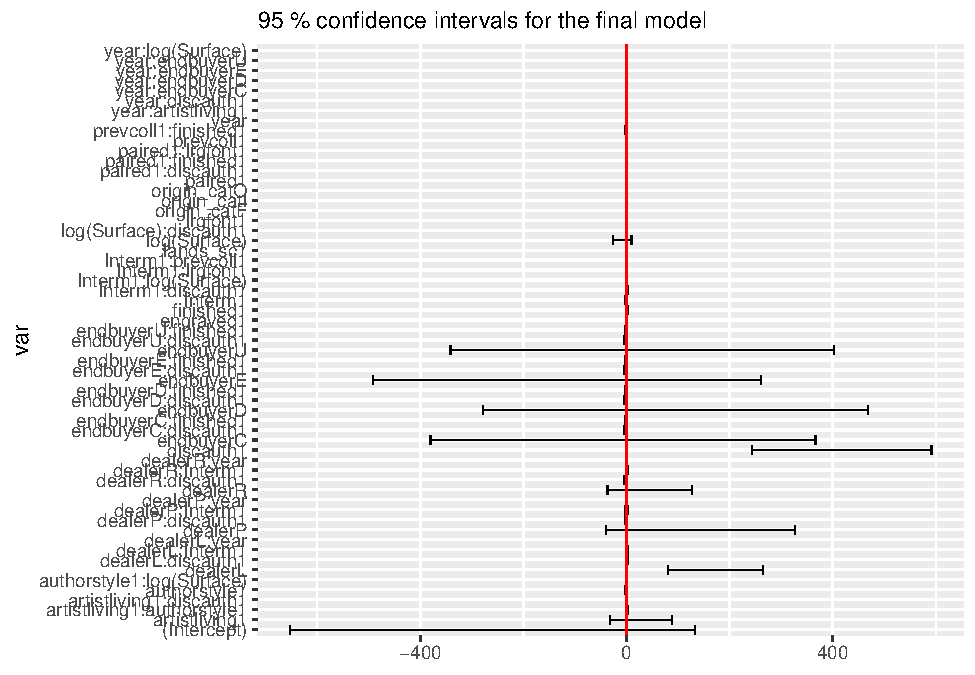
\includegraphics{Part-I-Writeup_files/figure-latex/unnamed-chunk-6-1.pdf}

\begin{Shaded}
\begin{Highlighting}[]
\NormalTok{paint_test_trans <-}\StringTok{ }\NormalTok{paint_test }\OperatorTok\StringTok{ }
\StringTok{  }\NormalTok{dplyr}\OperatorTok{::}\KeywordTok{select}\NormalTok{(}\OperatorTok{-}\KeywordTok{c}\NormalTok{(othartist, mytho, relig, landsALL)) }\OperatorTok
\StringTok{  }\NormalTok{dplyr}\OperatorTok{::}\KeywordTok{mutate}\NormalTok{(}\DataTypeTok{Surface =} \KeywordTok{log}\NormalTok{(Surface))}
\end{Highlighting}
\end{Shaded}

\hypertarget{summary-and-conclusions}{%
\subsubsection{4. Summary and
Conclusions:}\label{summary-and-conclusions}}


\end{document}
